% \pagebreak[4]
% \hspace*{1cm}
% \pagebreak[4]
% \hspace*{1cm}
% \pagebreak[4]

\chapter{Cơ sở lý thuyết} \label{theory-basis}

\ifpdf
    \graphicspath{{TheoryBasis/Chapter1Figs/PNG/}{TheoryBasis/Chapter1Figs/PDF/}{TheoryBasis/Chapter1Figs/}}
\else
    \graphicspath{{TheoryBasis/Chapter1Figs/EPS/}{TheoryBasis/Chapter1Figs/}}
\fi

Trong nội dung của chương này, đồ án sẽ trình bày về các kiến thức cơ bản cũng như như các thuật toán được sử dụng trong hệ thống tư vấn.
\section{Khảo sát các hệ tư vấn đã có}

Hệ thống tư vấn đã trở thành một đề tài khá phổ biến trong khoảng thời gian gần đây. Trong lĩnh vực xây dựng các hệ thống tư vấn trong quá khứ, người ta đã làm việc và nghiên cứu khá nhiều và ứng dụng rộng rãi trên các lĩnh vực khác nhau. Hầu hết công việc chủ yếu tập trung phát triền những phương pháp gợi ý những những đối tượng ưa thích đến cho người dùng. Ví dụ như những trang web gợi ý những bộ phim, gợi ý những quyển sách mà người dùng có thể yêu thích. Hệ thống tư vấn thông thường sẽ tiếp cận và giải quyết vấn đề theo 1 trong 2 hướng: Lọc dựa trên nội dung ( \textit{content-based filtering}) hoặc lọc cộng tác (\textit{collaborative filtering}). Tuy nhiên trên thực tế, việc áp dụng cả 2 hướng để giải quyết vấn đề cũng thường được cân nhắc trong việc giải quyết bài toán trong thực tế. (\textit{hybrid recommender system})

\subsection{Lọc cộng tác} là phương pháp được xây dựng dựa trên lý thuyết : "Những người có cùng hứng thú/mong muốn/sở thích về một vấn đề gì đó trong quá khứ thì có thể họ sẽ cũng có cùng hứng thú/mong muốn/sở thích trong tương lai". Ví dụ: hai người dùng A và B có chung sở thích ăn uống, họ đã mua các đồ ăn giống nhau. Nếu B còn thích thêm cả Cocacola nữa thì rất có thể A cũng thích, nên ta có thể gợi ý cho A mua thêm Cocacola. 

Phương pháp này thực hiện việc thu thập và đánh giá một lượng lớn thông tin về hành vi, sở thích của người dùng để tiên đoán sở thích của họ dựa trên sự giống nhau về thông tin giữa các người dùng. Ưu điểm của phương pháp này là nó không phải phụ thuộc vào việc nhận định, đánh giá để “hiểu được” nội dung của đối tượng tư vấn mà vẫn có thể đưa ra được kết quả thoả mãn mong muốn của người dùng. Tuy nhiên mặt hạn chế của phương pháp trên là nó cần một lượng lớn dữ liệu nguời dùng đa dạng để có thể hoạt động chính xác được. Và việc tính toán hành vi của từng người dùng cũng tiêu hao một lượng lớn tài nguyên máy tính.

\subsection{Lọc dựa trên nội dụng} là phương pháp mà người ta quân tâm đến 2 thực thể chính là người dùng và đối tượng được khuyến nghị đến cho người dùng. Quá trình lọc thực hiện bắt đầu từ việc xây dựng một hồ sơ người dùng (user profile) là tập các ưu tiên về sở thích của người dùng về đối tượng, và hồ sơ miêu tả đối tượng. Sau đó tiến hành lọc kết quả dựa vào phương pháp context-matching. Đây là phương pháp bắt nguồn từ lĩnh vực nghiên cứu triết xuất thông tin và lọc thông tin.

Hệ thống tư vấn trong tài liệu này áp dụng phương pháp lọc dựa trên nội dung, và cân nhắc thêm lọc cộng tác khi hệ thống đã phát triển sau này.


\section{Thuật toán Context-matching}
Thuật toán context-matching sử dụng để giải quyết bài toán cần Context-matching với Partial-matching ( khi mà khả năng đạt được “perfect match” là thấp ). Xây dựng các input context, output context và hàm đánh giá giữa các properties của chúng. Mục tiêu cuối cùng là một giá trị Boolean thể hiện sự phù hợp, hay không phù hợp của thực thể được tính đến.\\

Mô hình thuật toán được biểu diễn ở hình sau : 

\begin{figure}[!htbp]
  \begin{center}
    %\leavevmode
    \ifpdf
      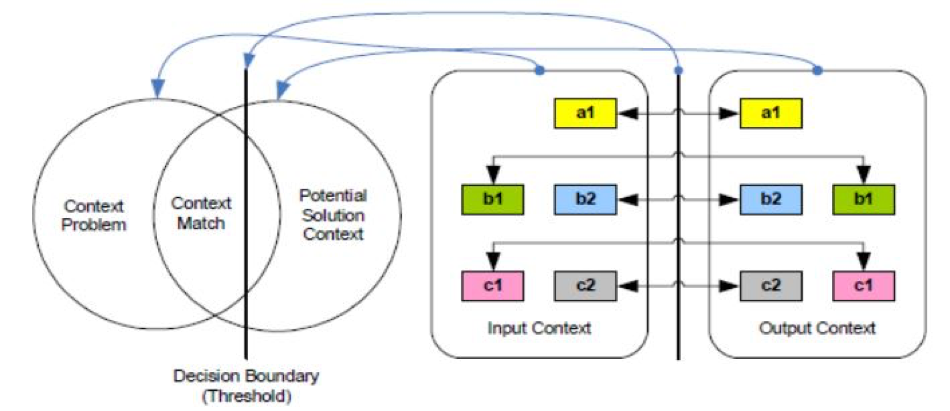
\includegraphics[scale=1]{contextmatch}
    \else
      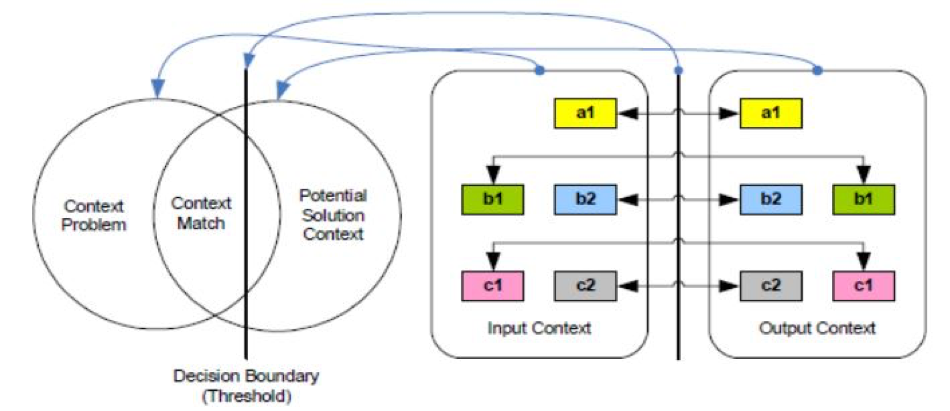
\includegraphics[scale=1]{contextmatch}
    \fi
    \caption{Mô hình thuật toán Context Matching }
    \label{ContextMatching}
  \end{center}
\end{figure}
\subsection{Tổng quan}	
Cấu trúc cơ bản của thuật toán là {ON <event> IF <condition> THEN <action>}. Trong đó <event> có thể là context data cần tính (event khởi động), hoặc là kết quả trả về của một lần so sánh ở phía trên, <condition> là cách so sánh giữa một input context property với một output context property sẽ được báo cáo dưới đây, <action> là kết quả của việc đánh giá trên <condition> và nó có thể là việc tiếp tục so sánh input và output tiếp theo hoặc là giá trị Boolean quyết định độ phù hợp của context (action cuối cùng).
\subsection{Input context và output context }	
Input context là nguyên mẫu để so sánh, các kết quả phù hợp là những kết quả phải có độ match với input context lớn nhất định. Output context là giải pháp tiềm năng cho vấn đề cần giải quyết trong bài toán, là một số lượng những thực thể đem so sánh với input context, được trích xuất từ cấu trúc dữ liệu. Từ input và output context, cần xây dựng một bộ các context properties là những thuộc tính bên trong quyết định context. Việc so sánh sẽ là so sánh giữa các context property.
\subsection{Các giá trị sử dụng}	
Giả sử áp dụng thuật toán cho bộ context properties [a1, b1, b2, c1, c2]. Ta có : 
\begin{itemize}
\item w: giá trị trong khoảng [0.10...1.00] phản ánh mức độ ưu tiên của thuộc tính 
\item e:  giá trị đánh giá xem thuộc tính ở input và output có match nhau không, e được biểu diễn trong khoảng [0...1]
\item av: (e * w) -  giá trị thực tế đánh giá độ match của thuộc tính, nằm trong khoảng  [0.00...1.00]
\item sav: av (a1) + av(b1) + av(b2) + av(c1) + av(c2) – tổng giá trị av 
\item mpv: giá trị sav cao nhất có thể đạt được. Nó thể hiện trường hợp mà tất cả các context property đều match nhau. 
\item rv: (sav / mpv) – giá trị trả về sau so sánh. Nó đánh giá tổng quan xem kết quả context match đến mức độ nào, nằm trong khoảng [0.00...1.00].  
\item t: giá trị cho ngưỡng đạt [0.10...1.00]. Context match  phù hợp khi so sánh ta có giá trị rv > t. 
 \end{itemize}
\subsection{Các bước thực hiện thuật toán }	
 \begin{itemize}
\item Bước 1: Đánh giá context match cho từng context property -> rút ra giá trị e . 
\item Bước 2: Thiết lập giá trị w đã được định sẵn cho từng context property
\item Bước 3: Tính giá trị av của thuộc tính av = (e* w)
\item Bước 4: Tính tổng các giá trị av của cả quá trình đánh giá (sav = (av (a1) + av (b1) + av (b2) + av (c1) + av (c2)))
\item Bước 5: Tính giá trị sav cao nhất có thể đạt (mpv = (w(a1) + w( b1) +w(b2) + w(c1) + w(c2)))
\item Bước 6: Tính giá trị kết quả trả về rv = (sav / mpv))
\item Bước 7: Sử dụng giá trị ngưỡng đã có sẵn để xác định xem output context có match với input context hay không . IF (rv) >= (t) THEN context-match = true [1] or IF (rv) < (t) THEN context-match = false [0]
 \end{itemize}
\section{Kỹ thuật Kansei Engineering}

\subsection{Tổng quan}

\subsection{Mô hình}
\subsubsection{Miền không gian Kansei}
\subsubsection{Miền không gian thuộc tính sản phẩm}
\subsubsection{Tổng hợp}



\section{Các cơ sở lý thuyết về công nghệ sử dụng}
\subsection{Firebase}
Firebase là một dịch vụ cơ sở dữ liệu thời gian thực hoạt động trên nền tảng đám mây được cung cấp bởi Google nhằm giúp các lập trình phát triển nhanh các ứng dụng bằng cách đơn giản hóa các thao tác với cơ sở dữ liệu.

Firebase hỗ trợ tối đa đối với những ứng dụng Backend, nó bao gồm các tiện ích lưu trữ dữ liệu, xác thực người dùng, static, hosting,… Vì thế giúp cho lập trình viên giảm thiểu công việc, và tập trung nâng cao trải nghiệm người dùng.\\

\textbf{Realtime Database – Cơ sở dữ liệu thời gian thực}
 
Firebase lưu trữ dữ liệu database dưới dạng JSON và thực hiện đồng bộ database tới tất cả các client theo thời gian thực. Cụ thể hơn là bạn có thể xây dựng được client đa nền tảng (cross-platform client) và tất cả các client này sẽ cùng sử dụng chung 1 database đến từ Firebase và có thể tự động cập nhật mỗi khi dữ liệu trong database được thêm mới hoặc sửa đổi.
 
 \begin{figure}[!htbp]
  \begin{center}
    %\leavevmode
    \ifpdf
      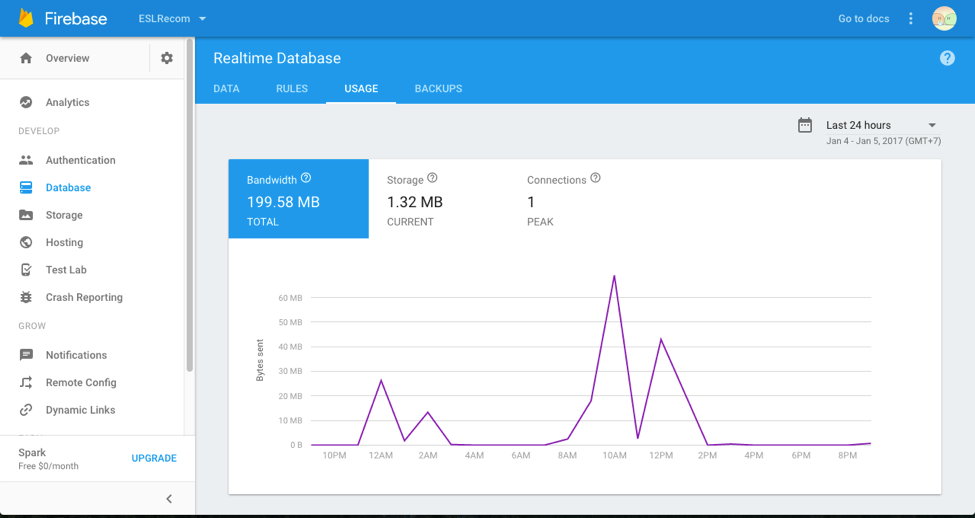
\includegraphics[scale=0.9]{firebasedb}
    \else
      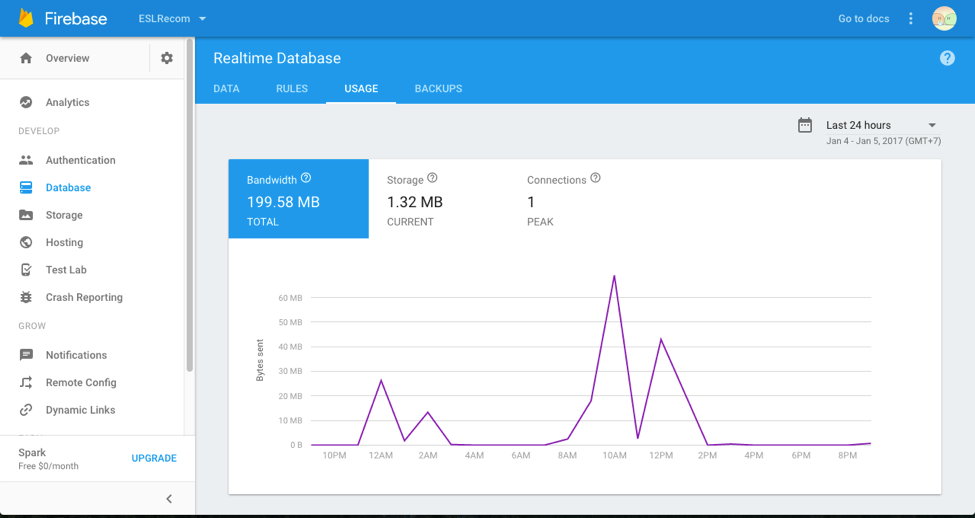
\includegraphics[scale=0.9]{firebasedb}
    \fi
    \caption{Cơ sở dữ liệu thời gian thực }
    \label{FirebaseDB}
  \end{center}
\end{figure}

 \begin{figure}[!htbp]
  \begin{center}
    %\leavevmode
    \ifpdf
      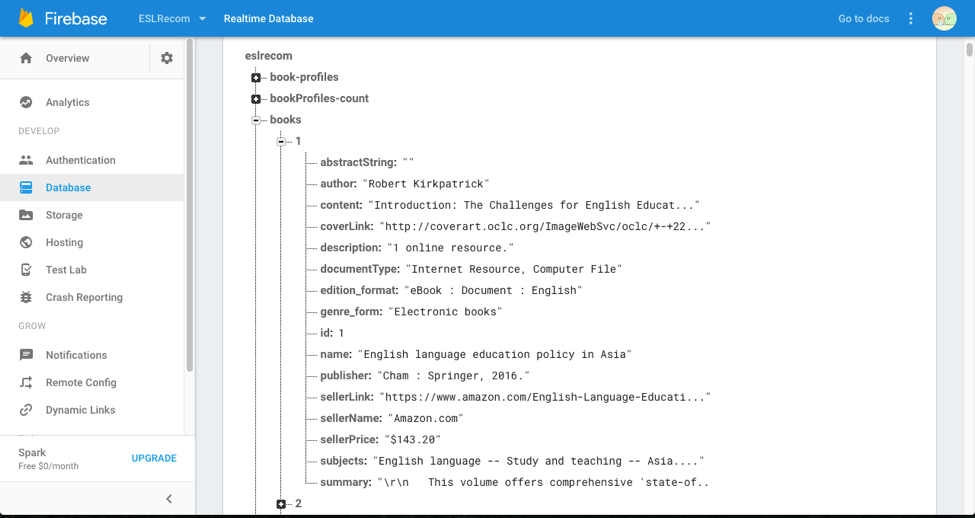
\includegraphics[scale=0.9]{firebasedb2}
    \else
      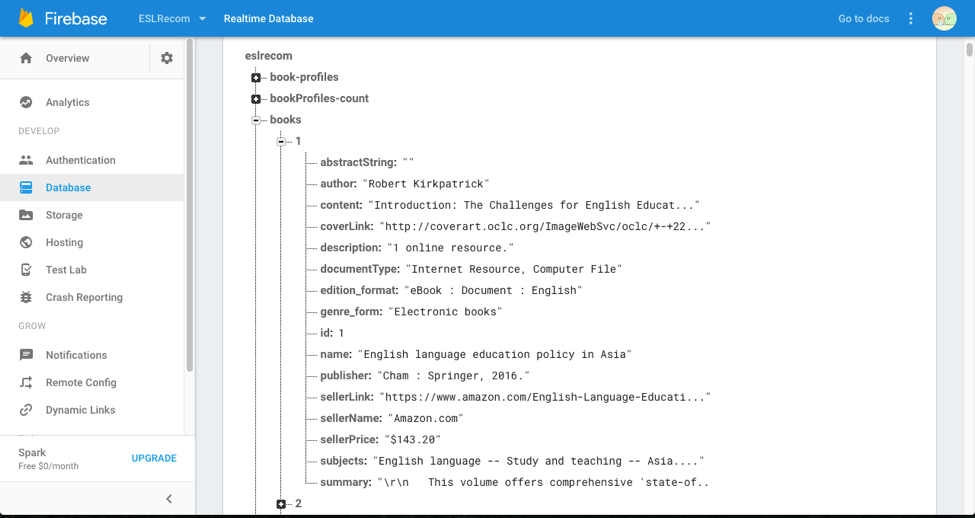
\includegraphics[scale=0.9]{firebasedb2}
    \fi
    \caption{Lưu trữ cơ sở tri thức chia sẻ giữa các thiết bị}
    \label{FirebaseDB2}
  \end{center}
\end{figure}

\subsection{Scrapy}

Scrapy là một framework được viết bằng Python, nó cấp sẵn 1 cấu trúc tương đối hoàn chỉnh để thực hiện việc crawl và extract data từ website một cách nhanh chóng và dễ dàng. Bạn muốn lấy dữ liệu từ các website nhưng dữ liệu đó quá lớn để copy rồi paste vào database của bạn, scrapy hỗ trợ bạn làm điều đó. Việc lấy dữ liệu website hoàn toàn tự động nhanh chóng và việc sử dụng scrapy cũng rất đơn giản giúp bạn tiếp kiệm được nhiều thời gian và công sức.

 \begin{figure}[!htbp]
  \begin{center}
    %\leavevmode
    \ifpdf
      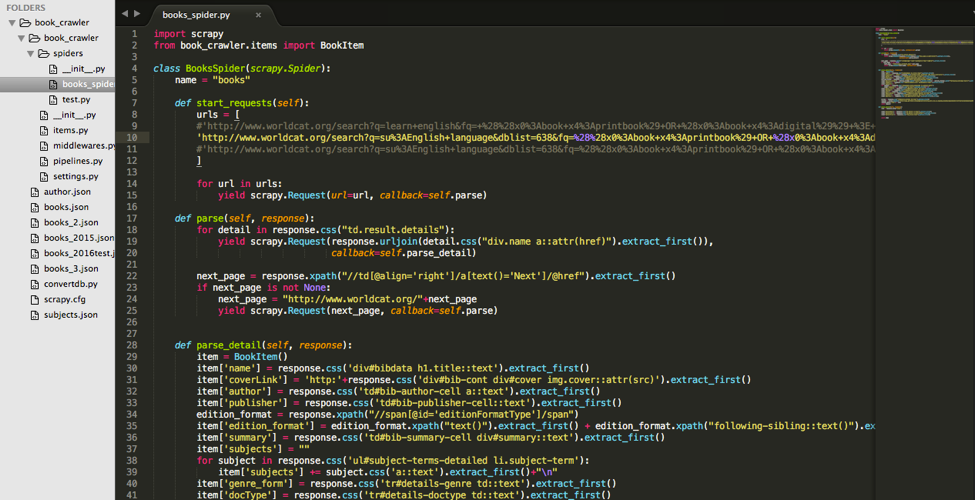
\includegraphics[scale=0.9]{scrapy}
    \else
      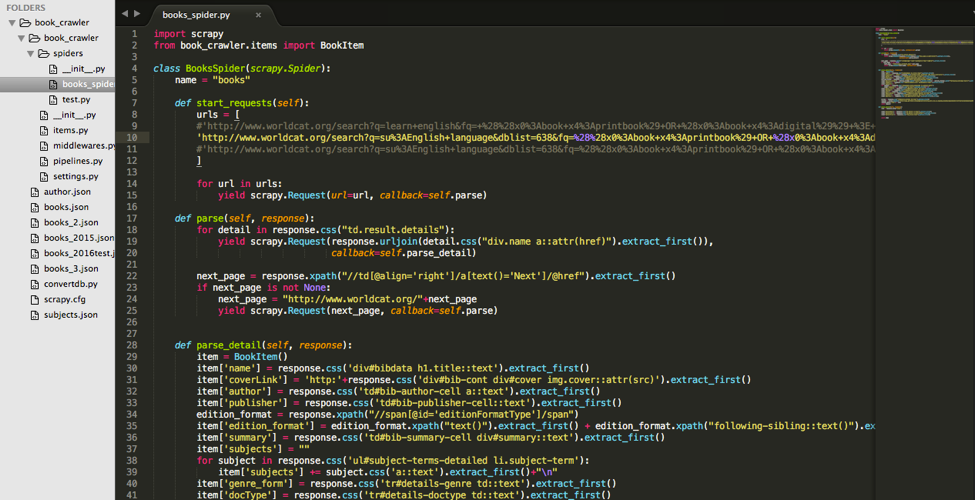
\includegraphics[scale=0.9]{scrapy}
    \fi
    \caption{Crawl tài liệu từ thư viện điện tử WorldCat.org }
    \label{Scrapy}
  \end{center}
\end{figure}

\subsection{Thuật toán tf-idf}

